% !TEX root = ../report.tex
\section{Das Partikelsystem}
\begin{Spacing}{\mylinespace}

Nachdem wir im ersten Projektsemester mit unserem CPU-basierten Partikelsystem sehr schnell an die Grenzen des machbaren gestoßen waren, haben wir uns im zweiten Projektsemester kurzfristig dafür entschieden, das System noch einmal komplett zu überarbeiten und dieses Mal auf eine reine GPU Implementierung zu setzen.

\subsection{Die Anforderungen}

Als Anforderungen haben wir uns gesetzt, ein hoch flexibles und vom restlichen System getrenntes Partikelsystem zu entwickeln, welches die Fähigkeit bietet mehrere hunderttausend oder sogar Millionen von Partikeln in Echtzeit darzustellen.  

\subsection{Die Umsetzung}

Um unser angestrebtes Ziel zu erreichen, haben wir auf eine Kombination aus verschiedenen Techniken gesetzt, die wir folgend etwas genauer Beschreiben werden.
 
\begin{description}
	\item[Billboarding] \hfill \\
	Für die Darstellung unserer Partikel haben wir zwei unterschiedliche Techniken in Betracht gezogen. Bei der erste und einfacheren Technik wird ein Partikel durch einen einzelnen Vertex repräsentiert und anschließend, als farbiger Punkt, auf den Bildschirm gezeichnet. Da wir aber nicht auf die Möglichkeit verzichten wollten, bei Bedarf unseren Partikeln auch eine Textur zuzuweisen, haben wir uns für die zweite, etwas aufwendigere, Technik das \textit{Billboarding} entschieden.
\\\\
\textit{Billboards} bestehen aus zwei dreieckigen Polygonen die ein Rechteck bilden (s. Abbildung \ref{fig:BBQuad}).	Dieses Rechteck wird anschließend im Vertexshader, mit Hilfe der Viewmatrix der Kamera, so transformiert damit es immer in Richtung des Betrachters ausgerichtet ist. Durch diese Eigenschaft, lassen sich, mit sehr geringem Rechenaufwand, unterschiedlichste Effekte realisieren. In unserem Anwendungsfall, die Darstellung von Rauch beziehungsweise Nebel. 

\begin{figure}[h!]
	\centering
	\vspace*{30px}
	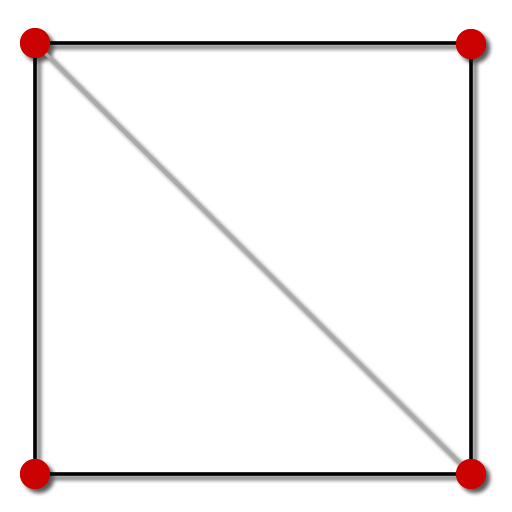
\includegraphics[width=110px]{graphics/billboardQuad.png}
	\caption{Aufbau des Rechtecks für ein Billboard.}
	\label{fig:BBQuad}
\end{figure}
\newpage
	\item[Instancing] \hfill \\
	Bei dieser Technik handelt es sich, um eine von der Grafikhardware bereitgestellten Funktionalität, zur Reduzierung von sogenannten \textit{Drawcalls}. Unter einem \textit{Drawcall} versteht man im Allgemeinen, das Zeichen eines Objekt mit einem bestimmten Material, einer Transformation und gegebenenfalls weiteren Eigenschaften. In unserem Fall wäre also jedes gezeichnete Partikel (Billboard) ein \textit{Drawcall}. Diese sind allerdings sehr teuer und bei der angestrebten Anzahl von über 1.000.000 Partikeln, wäre an eine Echtzeitfähigkeit nicht mehr zu denken gewesen. Somit entschieden wir uns für das \textit{Instancing}. Diese Technik erlaubt es 1.048.576 Instanzen der gleichen Geometrie, in unserem Fall die Billboards, in nur einem einzigen \textit{Drawcall} zu Zeichen. 
	
	\item[Rendertargets] \hfill \\
	In unserer vorherigen CPU-basierten Implementierung des Partikelsystems
	
\begin{figure}[h!]
	\centering
	\vspace*{30px}
	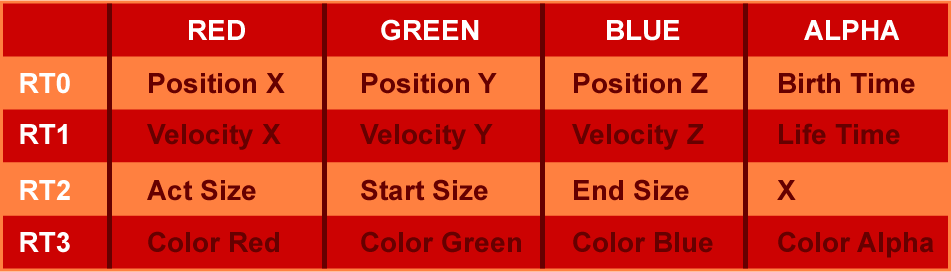
\includegraphics[width=410px]{graphics/RendertargetsChannels.png}
	\caption{Kanalbelegung der einzelnen Rendertargets.}
	\label{fig:RTCahnnels}
\end{figure}	
	
	\item[Ping-Pong] \hfill \\
	
\begin{figure}[h!]
	\centering
	\vspace*{30px}
	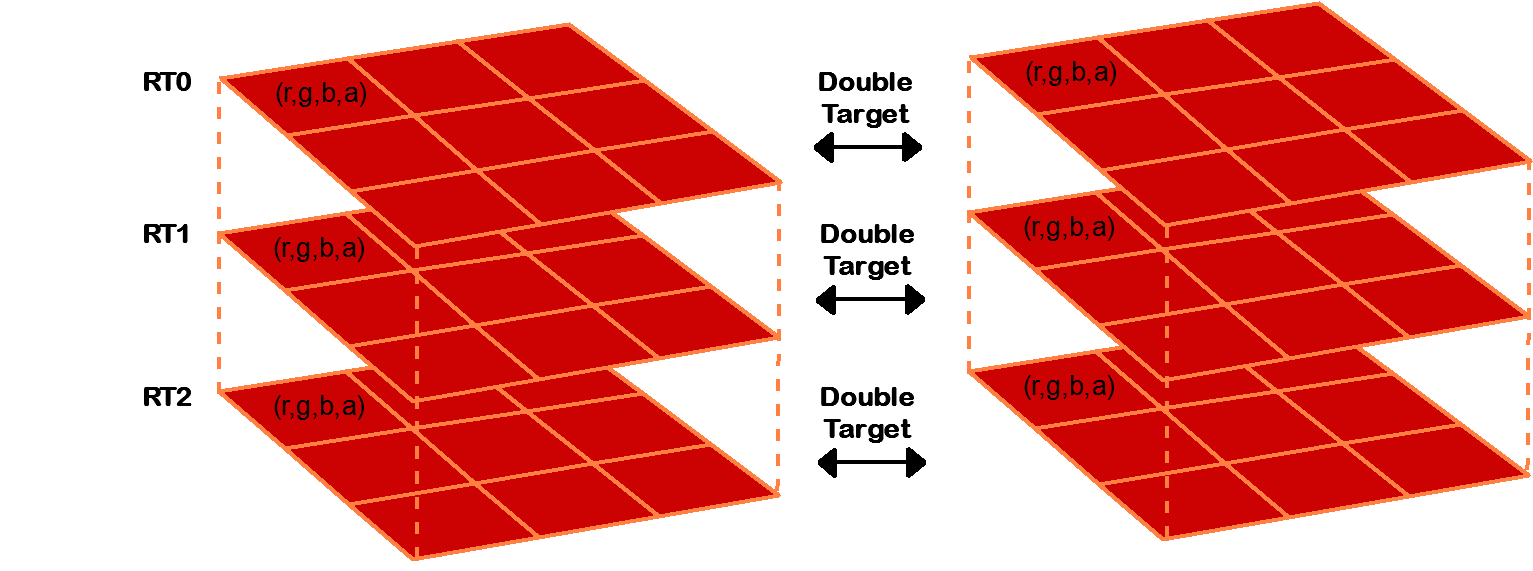
\includegraphics[width=410px]{graphics/DoubleTargets2.png}
	\caption{Double Rendertargets.}
	\label{fig:RTCahnnels}
\end{figure}
	\item[Alpha Blending] \hfill \\
\end{description}

Wie bereits im Kapitel der Datencontainer kurz ansgesprochen, besteht unser Partikelsystem aus verschiedenen Texturen (Rendertargets).
Manipuliert man nun eine dieser Texturen kommt es zu einem Konflikt, denn es werden die Texturen gleichzeitig manipuliert während sie dargestellt werden.
Um dennoch eine flüssige und fehlerfreie Darstellung zu erreichen dupliziert man die Texturen und manipuliert immer nur die Texturen die gerade nicht für die Visualisierung benötigt werden.

Durch die Duplizierung ist es nun einfach den beschriebenen Konflikt zu umgehen. Nachdem das erste Set der Rendertargets geupdatet wurde, wechselt man für die Aktualsierung einfach auf zweite Set (Swapping). Währenddessen kann die Visualisierung unabhängig auf dem anderen Set arbeiten ohne das Bildstörungen hervorzerufen werden.



\subsection{Das Ergebnis}

\end{Spacing}
\newpage
\clearpage
%% End Of Doc